\begin{figure*}[t!]
    \centering
        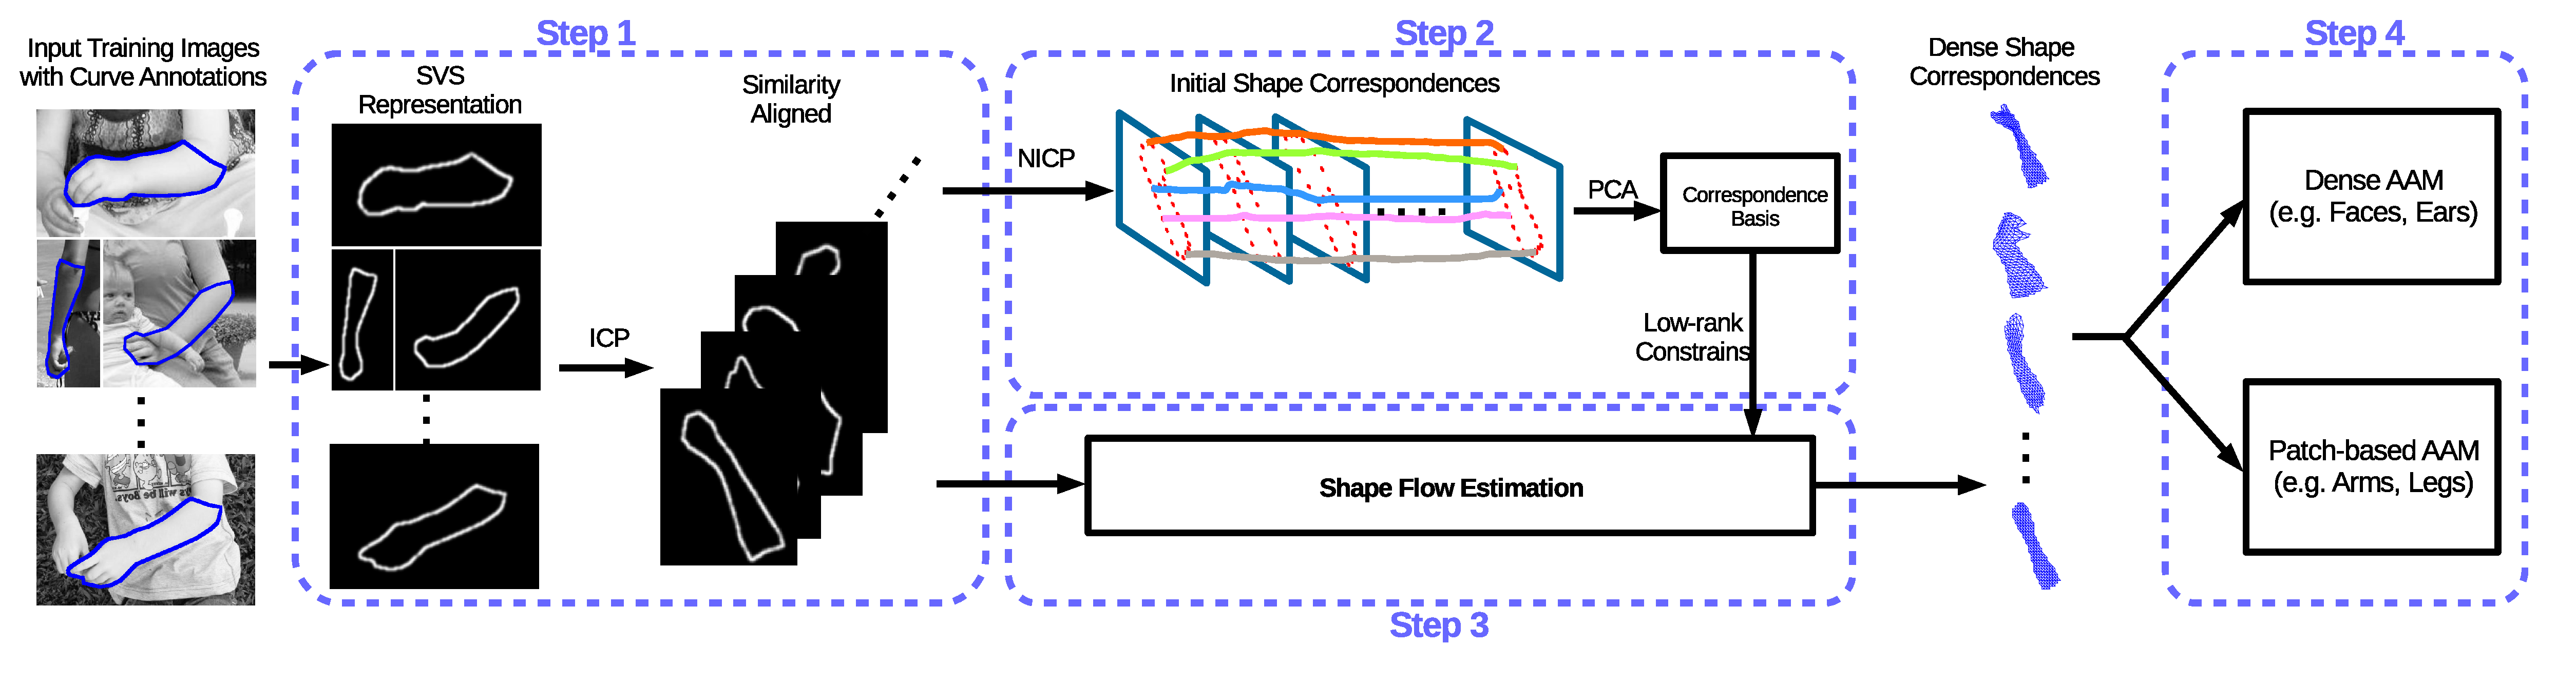
\includegraphics[width=\textwidth]{resources/architecture3}
    \caption{Schematic description of the proposed pipeline. Figure best viewed by zooming in.}
    \label{fig:archi}
\end{figure*}

\section{Constructing Deformable Models with Shape Flow}

% Deformable models are widely used for object detection, localization, recognition and tracking while training a deformable model with good generalisation requires tremendous amount of carefully annotated data, which is extremely time consuming. Even more, annotated data of a specific object category typically requires same numbers of landmarks for every training sample, making the annotation procedure significantly complex where corrext menual annotation of landmarks is impossible in various object classes e.g. ears.

% Despite the fact that that vast majority of existing methods are based on a sparse shape representation, dense shape representation reveals more nuanced structure in terms of [todo: explain].


This section presents the proposed method for establishing dense correspondences among training shapes 
by only using curve annotations.
%
%We propose a novel framework for building deformable models that does not require any consistent set of annotated landmarks and is based on a dense shape representation. Our method only requires a set of point or curve line annotations that does not need to be consistent over different training samples. 
%
%It combines the techniques of Non-rigid Iterative Closest Point (NICP) \cite{Amber2007}, multi-channel Support Vector Shape (SVS) \cite{Nguyen2013} representation and multi-image subspace flow \cite{Garg:2013hu} in an effective framework that has significant descriptive power.
%
It takes as input a set of training images of a particular object class, along with the corresponding curve annotations. The steps of our pipeline, which are also depicted in Figure~\ref{fig:archi}, are the following:

\noindent\textbf{Step 1:} Represent the curve annotations in a consistent way using a multichannel extension of the Support Vector Shape (SVS) representation \cite{Nguyen2013}. Apply the Iterative Closest Point (ICP) algorithm \cite{Besl1992} to achieve an initial alignment of the SVS images.

\noindent\textbf{Step 2:} Construct a correspondence basis for the training SVS images. This is acquired by applying Non-rigid ICP on the densely sampled annotated curves, followed by Principal Component Analysis (PCA).

\noindent\textbf{Step 3:} Establish dense correspondences between all the shapes in the training set by feeding the multichannel similarity-aligned SVS images into a multi-image subspace flow estimation.

\noindent\textbf{Step 4:} Utilise the dense correspondences acquired by the optical flow in order to automatically generate dense and sparse (on the outline) landmark annotations and build a dense \cite{ramnath2008increasing, Amberg2009, anderson2014using} and patch-based \cite{Tzimiropoulos2014} AAM, respectively.

The upcoming sections discuss each of the aforementioned steps in further detail.

%two major modules. The first module handles inconsistent annotation set by converting to landmark independent shape discriminator. While the other module produces shape flow on object discriminators to generate dense flow transformations in shape space following by robust PCA\cite{?} to generate deformable model. In this section, we present the entire architectures, design decision and algorithms.
\newcounter{steps}
{\refstepcounter{steps}\label{sec:step1}\subsection*{Step 1: Shape Representation Based on Support Vector Shapes}}
% \subsection{Shape Representation Based on Support Vector Shapes}
% \label{sec:step1}
%Ordinarily, construction of deformable model requires training data set having consistent number of landmarks. But unavoidable changes has to be made before applying same algorithm on diverse annotated data set.

In order to fully capture the variability among most deformable objects' shapes annotations, we use a representation based on Support Vector Shapes (SVS) \cite{Nguyen2013}. An SVS is a decision function trained on shapes using Support Vector Machines (SVMs) with Radial Basis Function (RBF) kernels. In this way, a shape is represented as a classifier function, which has several advantages: (a)~the representation is completely generic, e.g. it can be applied to sparse landmark points, curves lines or a combination of the two, and~(b) it fuses inconsistent landmarks into consistent and directly comparable decision functions. Furthermore, this representations is also robust against noise, missing data and outliers \cite{Nguyen2013}.

%In practice, we assume that all the training images correspond to the same object category and contain a set of inconsistent points and curve line annotations. 
The curve annotations for all training images are densely sampled to yield a set of landmarks per image, with this set being different for every training image. To train the SVM, these landmarks are assigned as belonging to the class with label `+1', whereas randomly sampled points around them are assigned as belonging to the class with label `-1'. Since the class `+1' has far less points than the class `-1', landmarks are assigned considerably larger weights so that $N_p \times W_p=N_n \times W_n$ where $N_p, N_n$ are number of points of the class `+1' and `-1' respectively and $W_p, W_n$ are their corresponding weights.

SVMs with RBF kernel function map any number of data points onto an infinite-dimensional space where positive and negative points are linearly separable, hence the classification boundary on 2D space represents the actual shape of the object. Note that the decision function for SVMs can be mathematically expressed as:
\begin{equation} \label{eq:decisionfunc}
    d(\bm{x})=\sum_i\alpha_i \, k(\bm{x}_i^*,\bm{x})
\end{equation}
where $\bm{x}_i^*$ are the so-called support vectors and \mbox{$k(\bm{x}, \bm{y}) = \exp\left(-\frac{\|\bm{x} -\bm{y}\|^2}{2 \sigma^2}\right)$} is the RBF kernel. The decision function $d(\bm{x})$ can be defined for every pixel $\bm{x}$ of the corresponding object image, therefore we interpret it as an image and we call it \emph{SVS image}.


Figure \ref{fig:build_svs} shows an exemplar shape representation of the human ear using SVS. As it can be observed, the final result does not drastically depend on the original number of annotated landmarks.


% \begin{figure}[b!]
%     \centering
%     \begin{subfigure}[b]{0.2\textwidth}
%             \includegraphics[width=\textwidth]{resources/landmark}
%         \caption{Spare landmarks}
%     \end{subfigure}
%     \qquad
%     \begin{subfigure}[b]{0.2\textwidth}
%             
\includegraphics[width=\textwidth]{resources/svs}
%         \caption{Decision function}
%         \label{fig:svs}
%     \end{subfigure}
%     \caption{Exemplar SVS shape representation. The decision function is trained on the set of sparse landmarks. In (b), brighter colour represents higher probability of a pixels belonging to the original shape.}
%     \label{fig:build_svs}
% \end{figure}

\begin{figure}[b!]
    \centering
    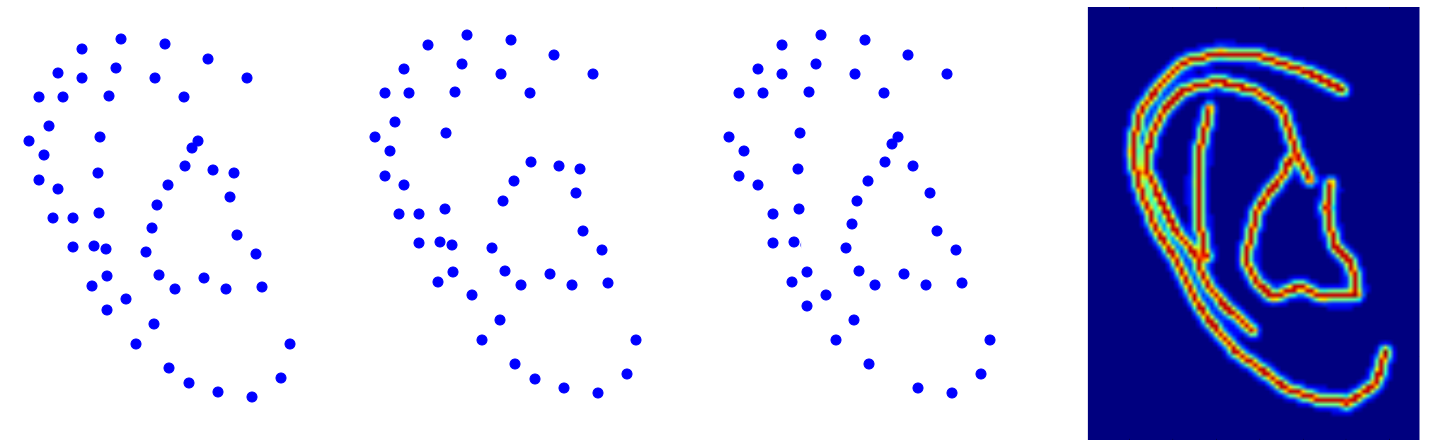
\includegraphics[width=0.4\textwidth]{resources/svs2}
    \caption{Exemplar SVS shape representation. A similar SVS image is obtained from different annotations of the same shape.}
    \label{fig:build_svs}
\end{figure}

We extend the SVS representation to support also the case where multiple curves with different labels are annotated. This is useful when annotating different structures of the same object, such as the curve of the left eyebrow and the curve of the right eyebrow on faces. Even though not absolutely necessary in our framework, it can provide further guidance on the estimation of dense shape correspondences for various object classes. In more detail, we create a multi-channel SVS image $\bm{d}(\bm{x})=[d_1(\bm{x}) \cdots d_i(\bm{x}) \cdots d_{N_c}(\bm{x})]$, where $d_i(\bm{x})$ is the SVS image that corresponds to the curve annotation of the $i$-th structure and $N_c$ is the total number of structures (a single curve annotation is the special case where $N_c=1$). Note that we do not necessarily require that all structures are annotated in all the object images: in the case that a structure is not annotated, the corresponding channel of the SVS image simply takes a zero value for all pixels. The shape flow estimation can deal with such missing information thanks to the spatial regularisation and the low-rank constraint that it adopts, c.f.~Step~\ref{sec:step3}.

After constructing the SVS representation for all images, the next step is to apply a simple similarity alignment over them. This is done because the goal here is to build a model capable of effectively representing non-rigid local shape deformations rather than global rotation, translation and scaling. The alignment is performed by using the Iterative Closest Point (ICP) algorithm \cite{Besl1992} on the annotated landmarks point cloud of the training images.


%\subsection{Correspondence Basis for Shape Flow Estimation}
{\refstepcounter{steps}\label{sec:step2}\subsection*{Step 2: Correspondence Basis for Shape Flow Estimation}}

We define the problem of shape flow as the joint estimation of optical flow fields between a reference SVS image and every SVS image of the training dataset, which yields dense correspondences across SVS images. This also defines for every training SVS image a warping function that registers it with the reference SVS image. To establish the dense correspondences robustly, we are inspired by the idea of subspace constraints in the estimation of multiframe optical flow \cite{Garg:2013hu}.

Instead of the \emph{motion} basis used in multiframe optical flow formulation of \cite{Garg:2013hu}, we build a \emph{correspondence} basis that introduces constraints on how points of different shapes are matched to each other. Every pixel of the reference SVS image is matched to its corresponding position at every training SVS image and in this way defines a \emph{correspondence vector}. This vector consists of the 2D locations of the specific point in all SVS images. To form this vector, the training images are arranged in an arbitrary order. Similarly to the order of training samples when Principal Component Analysis (PCA) is applied, this order does not affect the result of our method and any re-ordering would produce exactly the same results.


Formally, let $N_t$ be the number of training SVS images and $n=1,\ldots,N_t$ be the training image index. Also, let $\boldsymbol{q}_1(n),\ldots,\boldsymbol{q}_R(n):
\{1,\ldots,N_t\} \rightarrow \R^2$ be the $R$ orthonormal elements of the correspondence basis, where $\boldsymbol{q}_i(n)$ is the displacement vector that matches the points of the reference SVS image with the points of the $n$-th training SVS image, according to the variation described from the $i$-th correspondence basis element. Note that the basis elements $\boldsymbol{q}_i(n)$ are independent from the point location. Note also that the number of basis elements is typically much smaller than the full dimensionality ($2 N_t$) of correspondence vectors, therefore this basis plays a role of dimensionality reduction.


In addition, let $\Omega \subset \R^2$ be the image domain of the SVS images and $\bx$ denote the point location. We denote the shape flow result as $\bm{u}_n(\bx):\Omega\times \{1,\ldots,N_t\}
\rightarrow \R^2$,  where $\bm{u}_n(\bx)$ is the displacement vector that matches the point $\bx$ of the reference SVS image with its corresponding location at the $n$-th training SVS image.

Using the constructed correspondence basis, the shape flow can be approximated as:
\begin{equation}\label{eq:LinTrajModel}
    \bm{u}_n(\bx) \approx
    \sum_{i=1}^R\bm{q}_i(n)\bm{v}_i(\bx) \,\, ,
\end{equation}
where $\bm{v}_i(\bx)$ is the weight that needs to be applied on the $i$-th correspondence basis element, in order to get the correspondence vector for the point location $\bm{x}$. In other words, the shape flow for every point $\bm{x}$ is described as a linear combination of basis elements that is controlled by the coefficients $\bm{v}_i(\bm{x})$.
The values of the $i$-th coefficient for all the points $\bm{v}_i(\bm{x})$ can be interpreted as an image defined on $\Omega$. Using the correspondence basis, the determination of the shape flow boils down to the determination of the set of coefficients $\bm{v}_i(\bm{x})$. The above representation of shape flow, constrains the correspondence vectors to lie on a subspace and, therefore, acts as a low-rank prior that enforces coherency of the shape registration result over the whole training dataset of shapes.


The next section describes the methodology of constructing the correspondence basis and estimating the shape flow robustly.

% For all dense transformations $\bm{u}_n(\bm{x}), n \in \{1,...,F\}$, where $F$ is number of data and $\bm{x}$ is vector of pixels, Principle Component Analysis (PCA) is performed on trajectory to obtain low rank trajectory basis:
% \begin{equation}
%     \begin{bmatrix}
%         \bm{u_1}(\bm{x}) \\
%         \vdots \\
%         \bm{u_F}(\bm{x})
%     \end{bmatrix}
%     =
%     \begin{bmatrix}
%         \bm{q_1}(1) & \cdots & \bm{q_R}(1) \\
%         \vdots      & \ddots & \vdots  \\
%         \bm{q_1}(F) & \cdots & \bm{q_R}(F)
%     \end{bmatrix}
%     \times
%     \begin{bmatrix}
%         \bm{v_1}(x) \\
%         \vdots \\
%         \bm{v_R}(x)
%     \end{bmatrix}
% \end{equation}
% where $\bm{q_i}(n)$ are low rank components with $R \ll 2F$ and $\bm{v_i}(x)$ weighted each component with dependencies on $x$. Simpler expression shown below:
% \begin{equation}
%     \bm{u}_n(\bm{x})=\sum_{i=1}^R\bm{q_i}(n)\bm{v_i}(x)+\bm{\varepsilon_n}(\bm{x})
% \end{equation}

\begin{figure}[t!]
        \centering
        \begin{tabular}{ccc}
        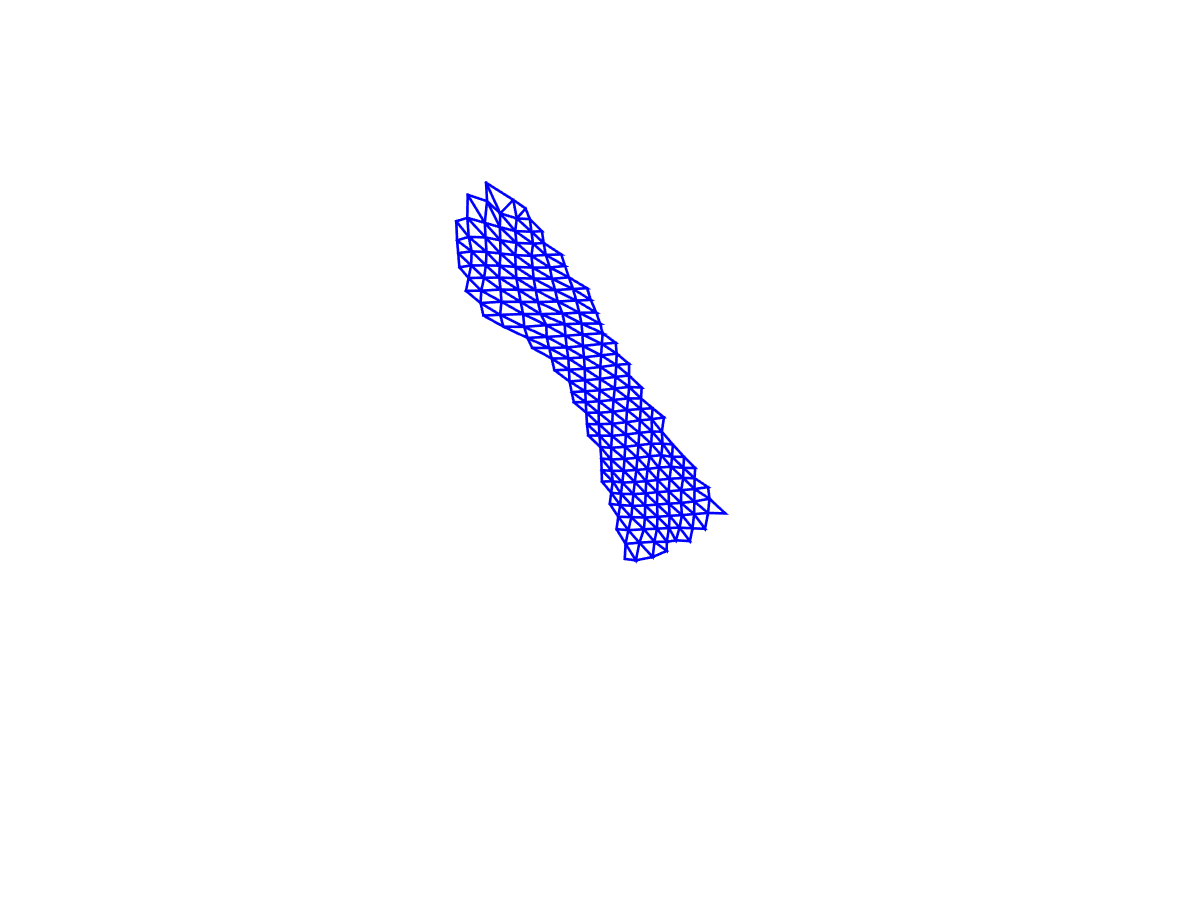
\includegraphics[trim=200 150 200 50,clip,width=.25\columnwidth]{resources/Fig_Flows/1}
        &
        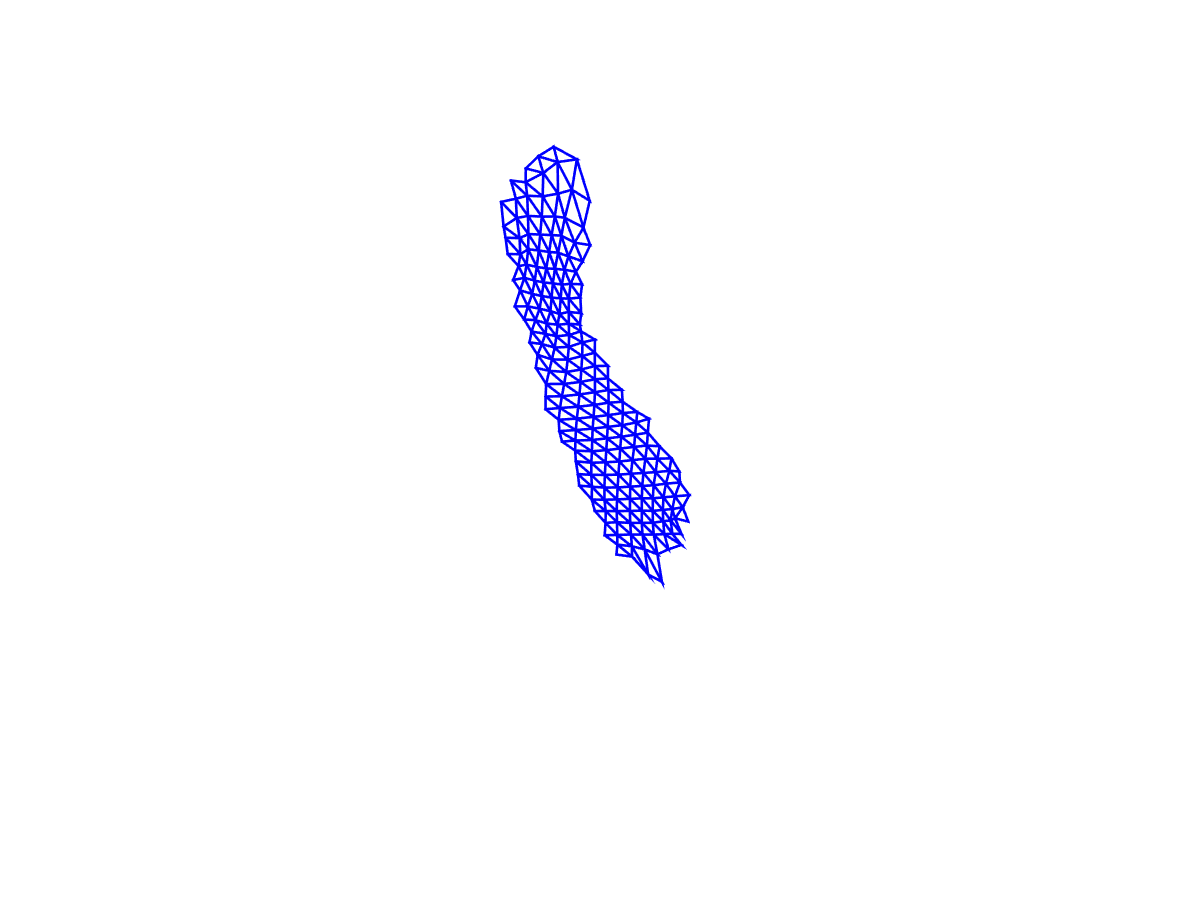
\includegraphics[trim=200 150 200 50,clip,width=.25\columnwidth]{resources/Fig_Flows/2}
        &
        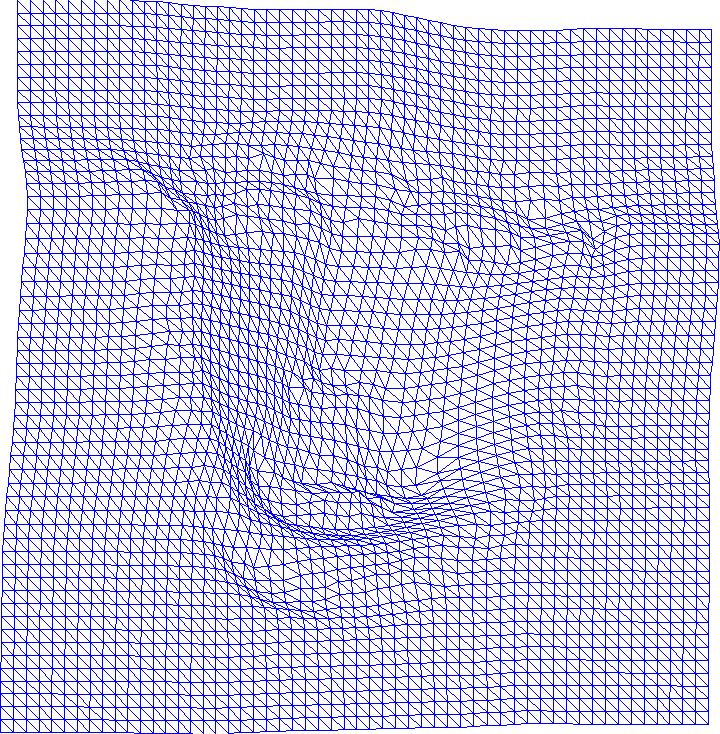
\includegraphics[trim=200 150 200 50,clip,width=.25\columnwidth]{resources/Fig_Flows/3}
        \\
        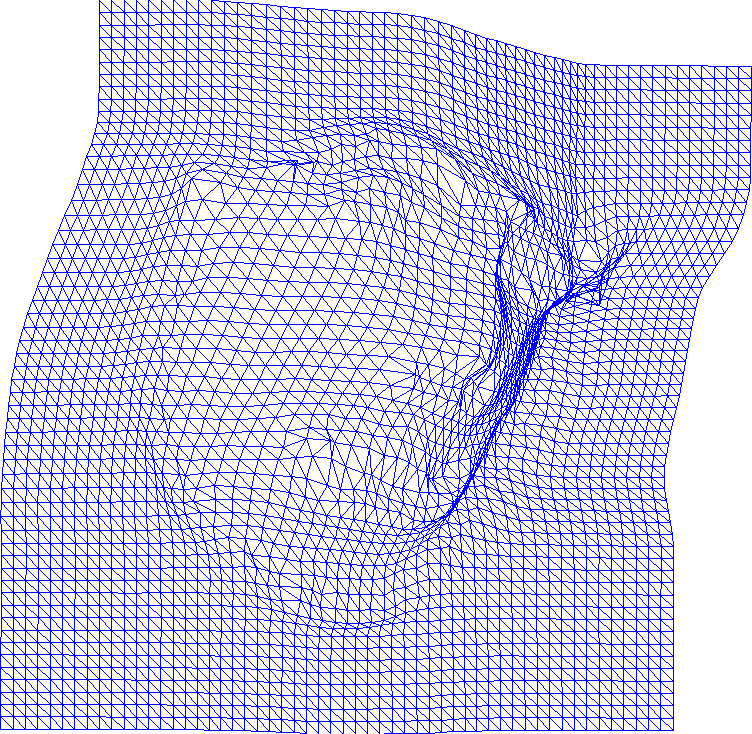
\includegraphics[trim=200 150 200 50,clip,width=.25\columnwidth]{resources/Fig_Flows/4}
        &
        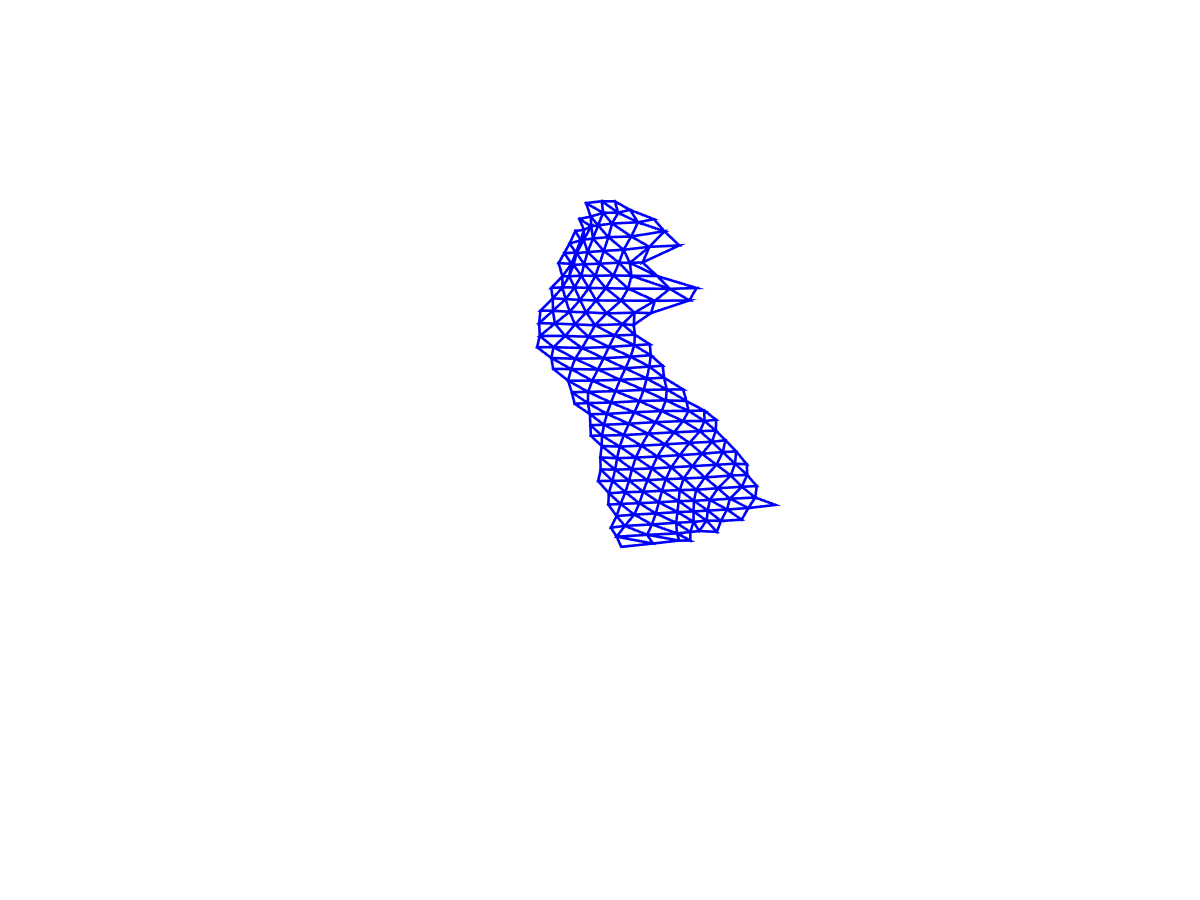
\includegraphics[trim=200 150 200 50,clip,width=.25\columnwidth]{resources/Fig_Flows/5}
        &
        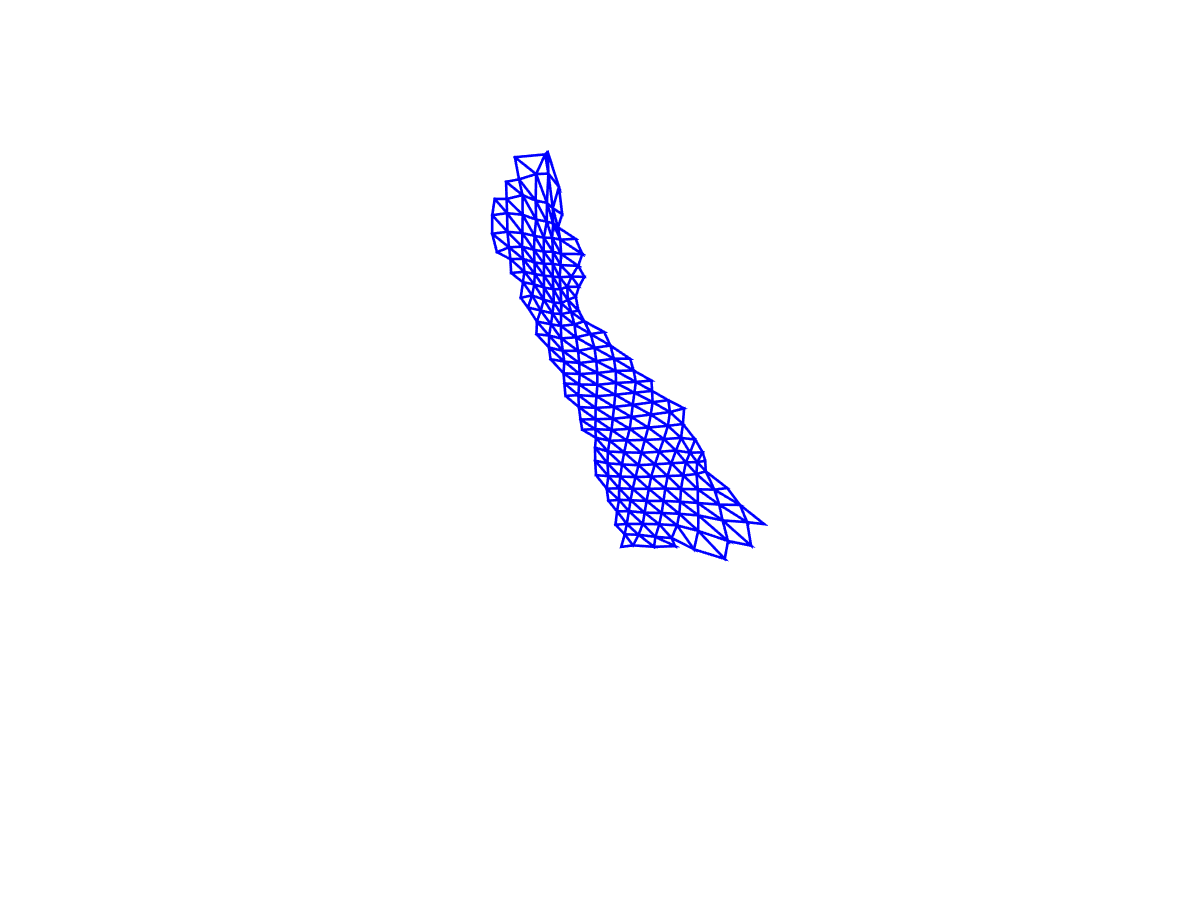
\includegraphics[trim=200 150 200 50,clip,width=.25\columnwidth]{resources/Fig_Flows/6}
        \end{tabular}
    \caption{Exemplar deformation fields for the left forearm, obtained using the proposed pipeline. Figure best viewed by zooming in.}
    \label{fig:deformationfield}
\end{figure}





% ---------------------------------------------------------------------------------------------------------------------------------------------------

{\refstepcounter{steps}\label{sec:step3}\subsection*{Step 3: Shape Flow Estimation}}
% \subsection{Shape Flow Estimation}
% \label{sec:step3}


%Using the SVS functions built from training data, one of the main steps of our pipeline is to estimate dense correspondences between all these functions. We propose to perform this estimation simultaneously for all training data, by using the correspondence basis. 

As already mentioned, our shape flow estimation builds upon robust methods for multiframe optical flow estimation \cite{Garg:2013hu}. However, optical flow estimation typically works based on the assumptions of brightness or colour constancy and motion smoothness, whereas in our setting the input training data correspond to shapes. For this reason, we propose to modify the formulation of \cite{Garg:2013hu} by using the correspondence basis that we introduced in conjunction with the SVS representation of shapes.


%
%In order to learn the such a subspace, we first transform the original annotation to point clouds. Then, we use NICP to align the previous point clouds with respect to a reference point cloud template. NICP iteratively deforms each point cloud until its points match the ones on the shape template and correspondences are established. However, because optical flow is a pixel-wise frame registration technique, we need to establish correspondences for all pixels on the reference frame rather than for sparse point clouds. To achieve this, we apply Thin Plate Spline (TPS) \cite{Bookstein1989} to find correspondences for all pixels in the reference frame given the point cloud correspondences provided by the previous NICP stage. Once dense correspondences have been established among all pixels, the so-called correspondence subspace is obtained by performing PCA the trajectory of all pixels. Note that incorporating the previous subspace as a low rank constrained in optical flow is consistent with its assumption of smooth motion.



\subsubsection*{Non-rigid ICP and Correspondence Basis Creation} \label{sec:trabasis}



To effectively build the correspondence basis, we first transform the original annotations to sparse point clouds. Then, we apply Non-rigid Iterative Closest Point (NICP)\cite{Amber2007} between the point cloud of annotations in the reference shape and the one of every shape of the training set. NICP iteratively deforms the cloud of points of every shape to match the points of the reference shape. This yields an initial estimation of the correspondence vectors on the sparse locations of annotated landmarks on the reference shape. Finally, the correspondence basis is found by applying PCA on these  correspondence vectors and keeping only the first $R$ principal components.

%To make this correspondence vectors estimation dense (i.e.~for every pixel of the reference SVS image), we apply Thin-Plate Splines (TPS)\cite{Bookstein1989} interpolation. Finally, the correspondence basis is found by applying PCA on the result of TPS interpolation and keeping only the first $R$ principal components.




%
%
%Since optical flow pixel-wise frame registration, the trajectory basis build should also match the dimension, which is dense on shapes with trajectory length depends on number of training data. With correspondences produced after applying NICP, Thin-Plate Spline (TPS)\cite{Bookstein1989} transformations are utilized to warp every shape planes to template plane thereby generates an implicit dense shape registering. For all dense transformations $\bm{u}_n(\bm{x}), n \in \{1,...,F\}$, where $F$ is number of data and $\bm{x}$ is vector of pixels, Principle Component Analysis (PCA) is performed on trajectory to obtain low rank trajectory basis:
%\begin{equation}
%    \begin{bmatrix}
%        \bm{u_1}(\bm{x}) \\
%        \vdots \\
%        \bm{u_F}(\bm{x})
%    \end{bmatrix}
%    =
%    \begin{bmatrix}
%        \bm{q_1}(1) & \cdots & \bm{q_R}(1) \\
%        \vdots      & \ddots & \vdots  \\
%        \bm{q_1}(F) & \cdots & \bm{q_R}(F)
%    \end{bmatrix}
%    \times
%    \begin{bmatrix}
%        \bm{v_1}(x) \\
%        \vdots \\
%        \bm{v_R}(x)
%    \end{bmatrix}
%\end{equation}
%where $\bm{q_i}(n)$ are low rank components with $R \ll 2F$ and $\bm{v_i}(x)$ weighted each component with dependencies on $x$. Simpler expression shown below:
%\begin{equation}
%    \bm{u}_n(\bm{x})=\sum_{i=1}^R\bm{q_i}(n)\bm{v_i}(\bm{x})+\bm{\varepsilon_n}(\bm{x})
%\end{equation}
%Although optical flow on shapes made under the assumption that objects motion are smooth, the low rank constrain on trajectory basis recovered the hypothesis.

% \begin{figure}[t!]
%         \centering
%         \begin{tabular}{cccccccc}
%         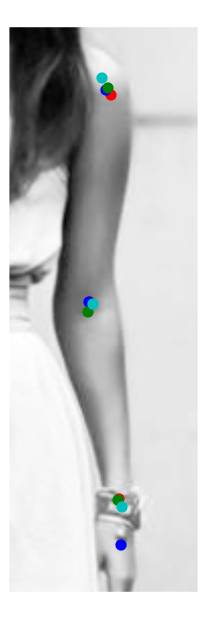
\includegraphics[trim=200 150 200 50,clip,width=.1\columnwidth]{resources/Fig_Variance/image_0}
%         &
%         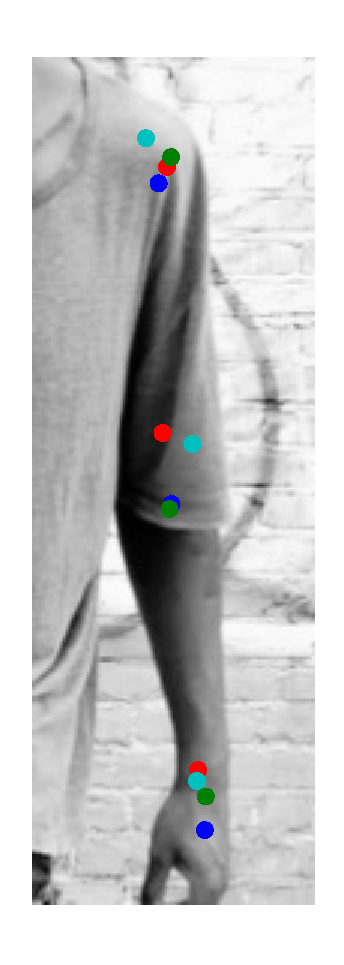
\includegraphics[trim=200 150 200 50,clip,width=.1\columnwidth]{resources/Fig_Variance/image_1}
%         &
%         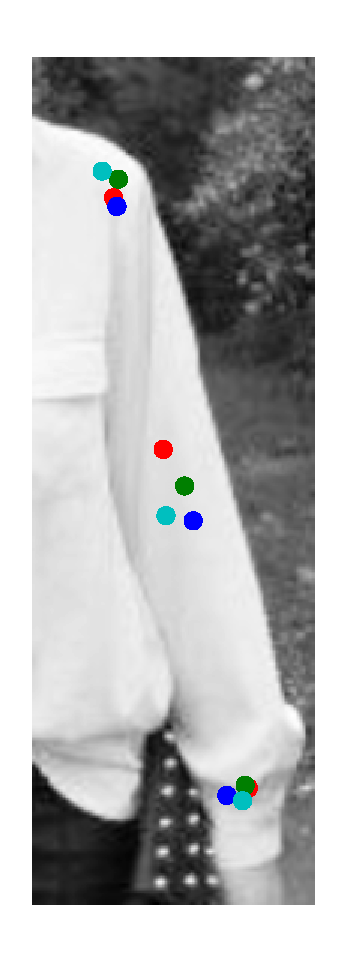
\includegraphics[trim=200 150 200 50,clip,width=.1\columnwidth]{resources/Fig_Variance/image_2}
%         &
%         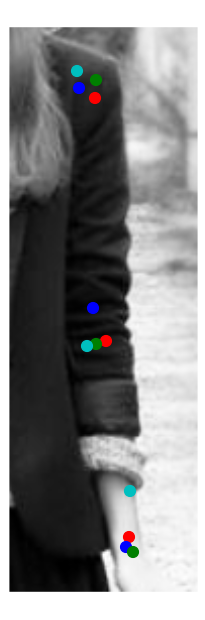
\includegraphics[trim=200 150 200 50,clip,width=.1\columnwidth]{resources/Fig_Variance/image_3}
%         &
%         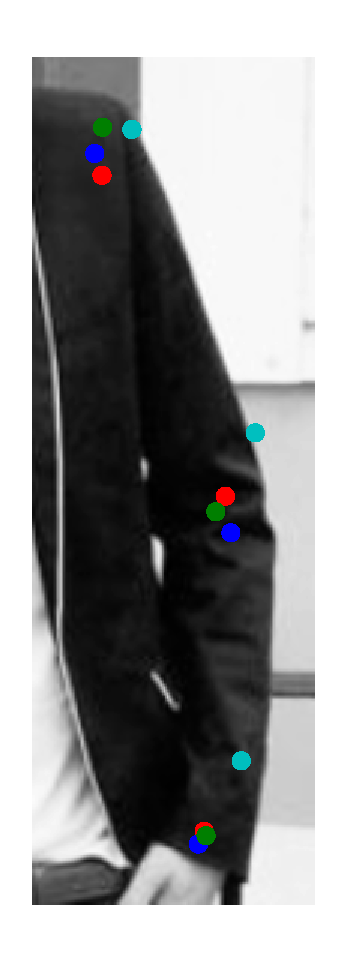
\includegraphics[trim=200 150 200 50,clip,width=.1\columnwidth]{resources/Fig_Variance/image_4}
%         &
%         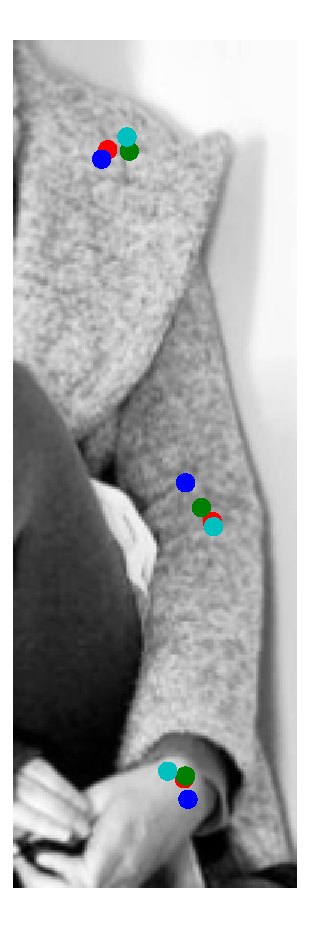
\includegraphics[trim=200 150 200 50,clip,width=.1\columnwidth]{resources/Fig_Variance/image_5}
%         &
%         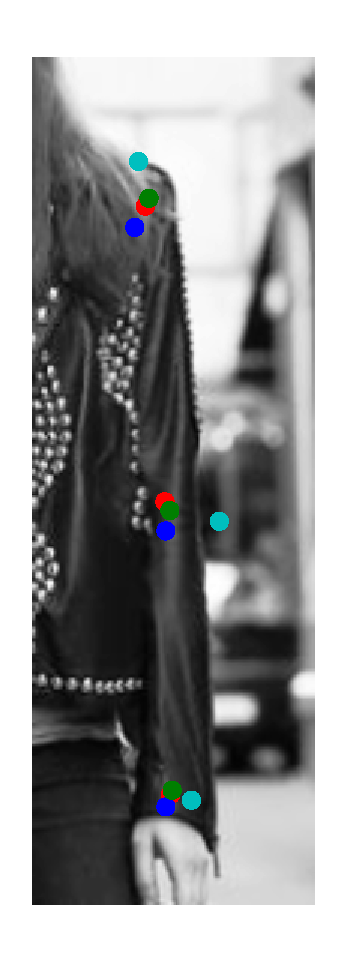
\includegraphics[trim=200 150 200 50,clip,width=.1\columnwidth]{resources/Fig_Variance/image_6}
%         &
%         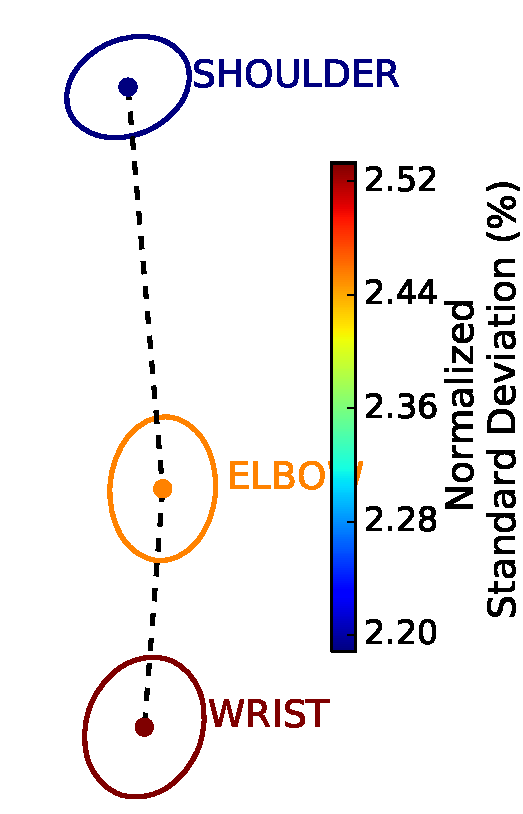
\includegraphics[trim=200 150 200 50,clip,width=.1\columnwidth]{resources/Fig_Variance/variances}
%         \end{tabular}
%     \caption{Variances}
%     \label{fig:variances}
% \end{figure}




\subsubsection*{Variational Shape Flow Estimation}%{Multi-image Subspace Flow}
\label{varshapeflow}


Let $\bm{d}(\bx;n)$, $\bm{d}(\bx;0):\Omega\rightarrow \R^{N_c}$ be the $n$-th training SVS image and the reference SVS image respectively. Following \cite{Garg:2013hu}, we propose to estimate the shape flow over all training images by minimizing the following energy:
\begin{align}
E_{sf} & =\alpha
\int_{\Omega}\sum_{n=1}^{N_t} \|\bm{d}(\bx+\bm{u}_n(x);n)-\bm{d}(x;0)\| \ud \bx \label{eq:costfunc}\\
    &+ \beta \int_{\Omega}\sum_{n=1}^{N_t}\|\bm{u}_n(\bx)-\sum_{i=1}^R\bm{q}_i(n)\bm{v}_i(\bx)\|^2 \ud \bx \label{eq:lowrank}\\
    &+
\int_\Omega  \sum_{i=1}^R \,\, \left \|    \nabla \bm{v}_i(\bx)    \right \|  \,\ud \bx \label{eq:TVterm}
\end{align}
This energy consists of two sets of unknown shape flows that are relatively close to each other: (i) $\bm{u}_n(x)$ which tries to explain the data from the input SVS images, and (ii) the shape flow determined by the correspondence basis coefficients $\bm{v}_i(\bx)$ that are spatially regularised and enforce a low-rank prior. We minimize this energy jointly with respect to $\bm{u}_n(\bx)$ and $\bm{v}_i(\bx)$. The positive parameters $\alpha$ and $\beta$ weigh the balance between the terms of the energy.

The \textbf{first term} of the above energy \eqref{eq:costfunc} is a data attachment term
that uses the robust $\Lone$-norm.  It is based on the assumption that the values of the reference SVS image $\bm{d}_0(\bx)$ at every pixel $\bx$ are preserved at its corresponding locations on all training SVS images $\bm{d}_n(\bx)$. The use of an $\Lone$-norm improves the robustness of the method since it allows deviations from this assumption, which might occur in practice.
The \textbf{second term} of the energy \eqref{eq:lowrank} penalizes the difference between the two sets  of shape flows and acts as a coupling term between them.
The \textbf{third term} of the energy \eqref{eq:TVterm} corresponds to the spatial Total Variation regularization \cite{rudin92} of
the correspondence basis coefficients $\bm{v}_i(\bx)$.
This term penalizes spatial oscillations of each coefficient caused by distortions of the SVS images but not strong discontinuities that are desirable in the borders of different object regions. In addition, this term allows to fill in information into regions where the shape information in the SVS images is missing, due to e.g.~regions with no annotations.

We implement the minimization of the energy $E_{sf}$ by using the optimization algorithm described in \cite{Garg:2013hu}. In every coarse-to-fine and warping iteration, we use an initialization that comes from the previous iteration and for the very beginning, we initialize with the shape flow result of the TPS interpolation described in Sec.~\ref{sec:trabasis}. We approximate the data term \eqref{eq:costfunc} by linearizing the SVS images around the initialization. After that, the energy becomes convex and we optimize it using alternating optimization w.r.t.~$\bm{v}_i(\bx)$ and $\bm{u}_n(\bx)$. The minimization w.r.t.~
$\bm{v}_i(\bx)$ is decoupled for every coefficient $i$ and corresponds to Rudin-Osher-Fatemi Total Variation denoising \cite{rudin92}, which we solve efficiently by applying the first order primal-dual algorithm of \cite{Chambolle:Pock:JMIV2011}. The minimization w.r.t.~
$\bm{u}_n(x)$ is decoupled for every pixel $\bx$ and every shape index $i$. This minimization is also implemented by applying the efficient primal-dual algorithm of \cite{Chambolle:Pock:JMIV2011}.



Figure~\ref{fig:deformationfield} shows some examples of deformation fields derived from the estimated shape flow computed by the aforementioned method. These results correspond to exemplar training shapes in the case of an arm dataset.


%
%
%To register all decision functions to temp`late shape, decision function $d_i(\bm{x}), i \in {1,...,F}$ are grouped into one sequence before applying flow algorithm. The objective cost function we would like to minimise is:
%\begin{align}
%    \operatorname*{arg\,min}_{\bm{u}_n(\bm{x}), \bm{v}}&=\alpha \int_{\Omega}\sum_{n=1}^F|\bm{d_n}(x+\bm{u}_n(x))-\bm{d_0}(x)\| dx  \label{eq:costfunc}\\
%    &+ \beta \int_{\Omega}\sum_{n=1}^F\|\bm{u}_n(x)-\sum_{i=1}^R\bm{q_i}(n)\bm{v_i}(x)\|^2 dx \label{eq:lowrank}\\
%    &+ \sum[\bm{TV}(Qv)]
%\end{align}
%where $d_n(x)$ is the decision function from~\eqref{eq:decisionfunc}, which returns possibilities of given coordinate classified as shape component where coordinates are from set $\Omega \in \Re^2$. $TV(Qv)$ is total variation as regularization on low rank subspace, $Q$ is trajectory basis and $v^T.L.v$ is low rank spacial constrains.
%
%Term~\eqref{eq:costfunc} state the shape constancy where points having similar classification probability are from same object.
%Part~\eqref{eq:lowrank} applies constrain on low rank trajectory basis states in section~\ref{sec:trabasis}.
%The objective cost function has two free parameters $u$ and $v$, so we perform alternating minimisation. The equation can be solved using a thresholding scheme after linearisation of image functions. The minimisation can be speed up by paralleling the minimisation for every spatial-temporal point $(x;n), x \in \Omega, n \in \{1,...F\}$ independently.
%
%
%
%
%
%
%After solving the equation, $\bm{u}_n(\bm{x}), x \in \Omega$ gives a group of deformation fields that registering every decision functions in the shape sequence to reference frame e.g. $\bm{u_1}(\bm{x})$ registers decision function $\bm{d_1}(\bm{x})$ to the reference frame. Figure~\ref{fig:deformationfield} demonstrates deformation fields that warps from reference frame where there is no deformation.

% \begin{figure}[h!]
%     \centering
%         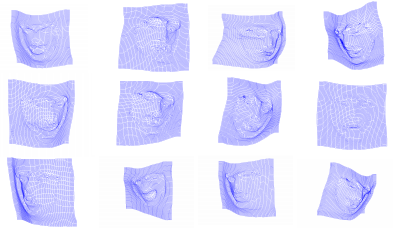
\includegraphics[width=0.5\textwidth]{resources/df}
%     \caption{Deformation field built}
%     \label{fig:deformationfield}
% \end{figure}



% Applying PCA on deformations trains dense deformable shape model:
% \begin{equation*}
%     \bm{s_p}=\bm{\bar{s}} + \bm{U}_s\bm{p}
% \end{equation*}
% where $\bm{s_p}$ is deformed shape instance. $\bm{\bar{s}}$ is mean shape and $\bm{U}_s\bm{p}$ are eigenvectors with corresponding parameters $p$. Figure~\ref{fig:models} shows an instance of deformed shape and appearance model.
% \begin{figure}[h!]
%     \centering
%     \begin{subfigure}[b]{0.22\textwidth}
%             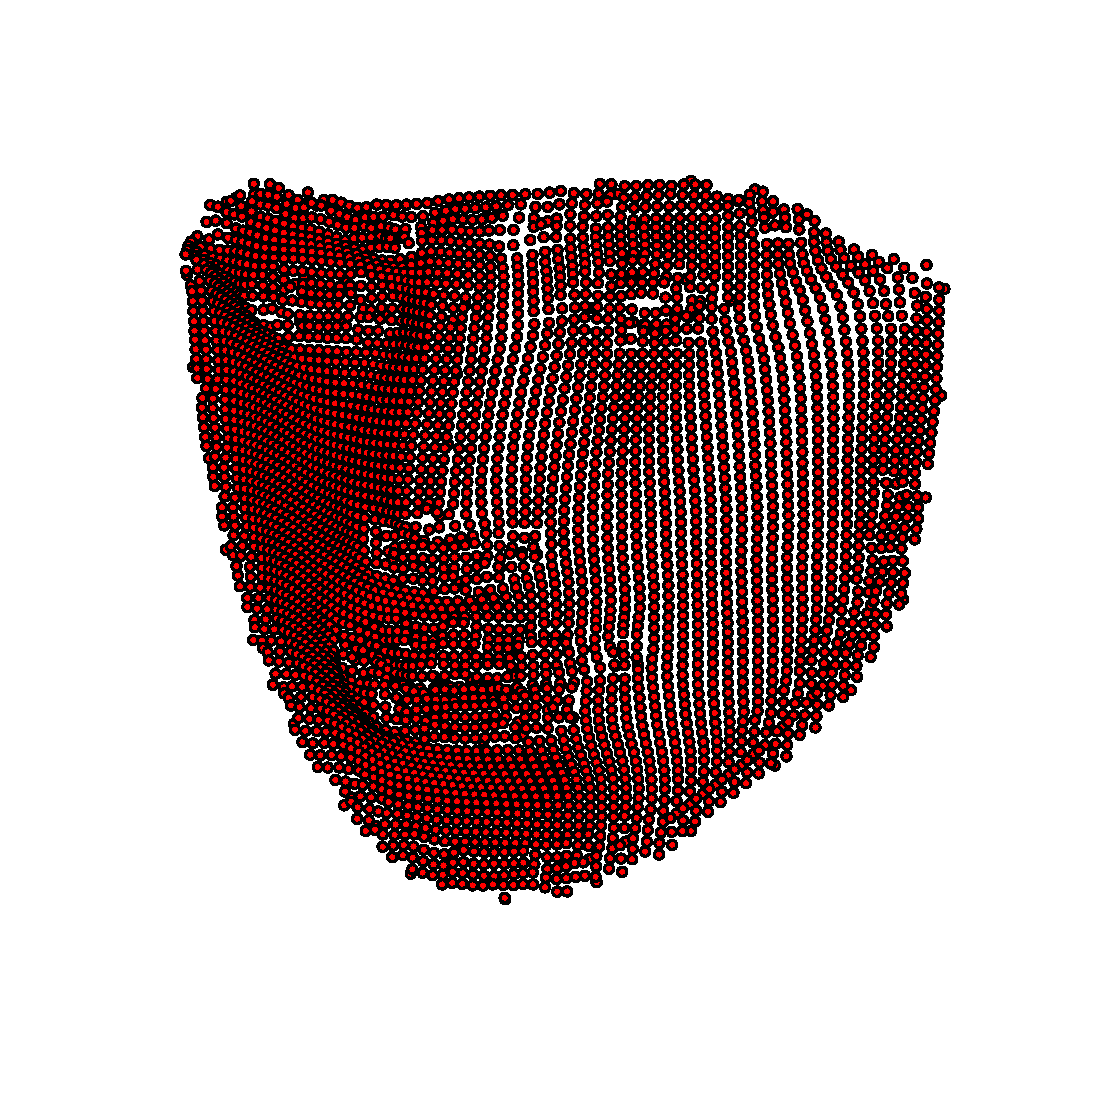
\includegraphics[width=\textwidth]{resources/Fig_dAAM/of_shape}
%     \end{subfigure}
%   	\hfill
%     \begin{subfigure}[b]{0.22\textwidth}
%             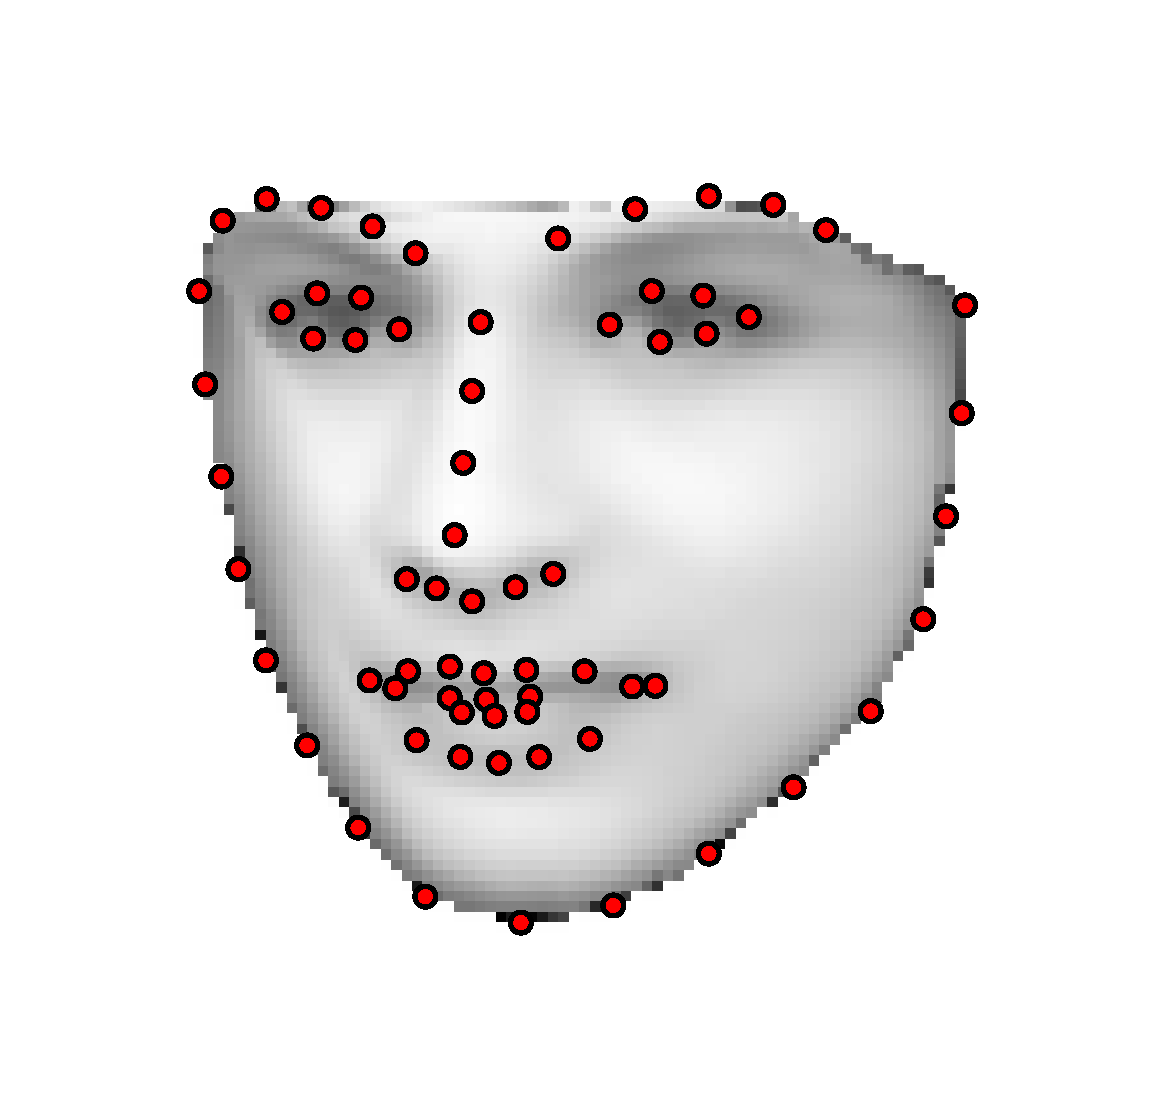
\includegraphics[width=\textwidth]{resources/Fig_dAAM/of_app}
%     \end{subfigure}
%     \caption{Dense Deformable Model}
%     \label{fig:models}
% \end{figure}

% \begin{figure}[h!]
%     \centering
%     \begin{subfigure}[b]{0.22\textwidth}
%             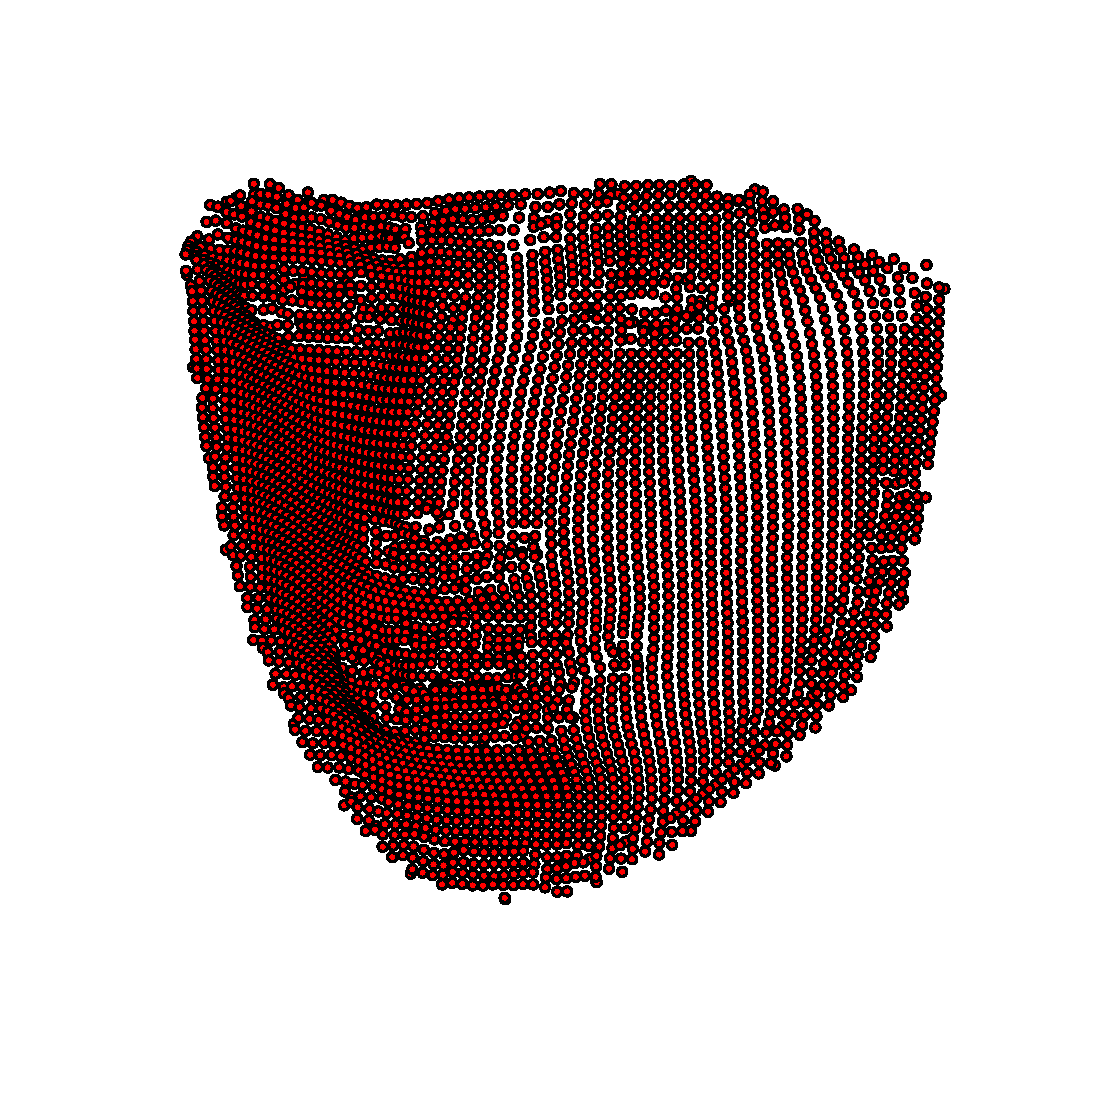
\includegraphics[width=\textwidth]{resources/Fig_dAAM/of_shape}
%     \end{subfigure}
%   	\hfill
%     \begin{subfigure}[b]{0.22\textwidth}
%             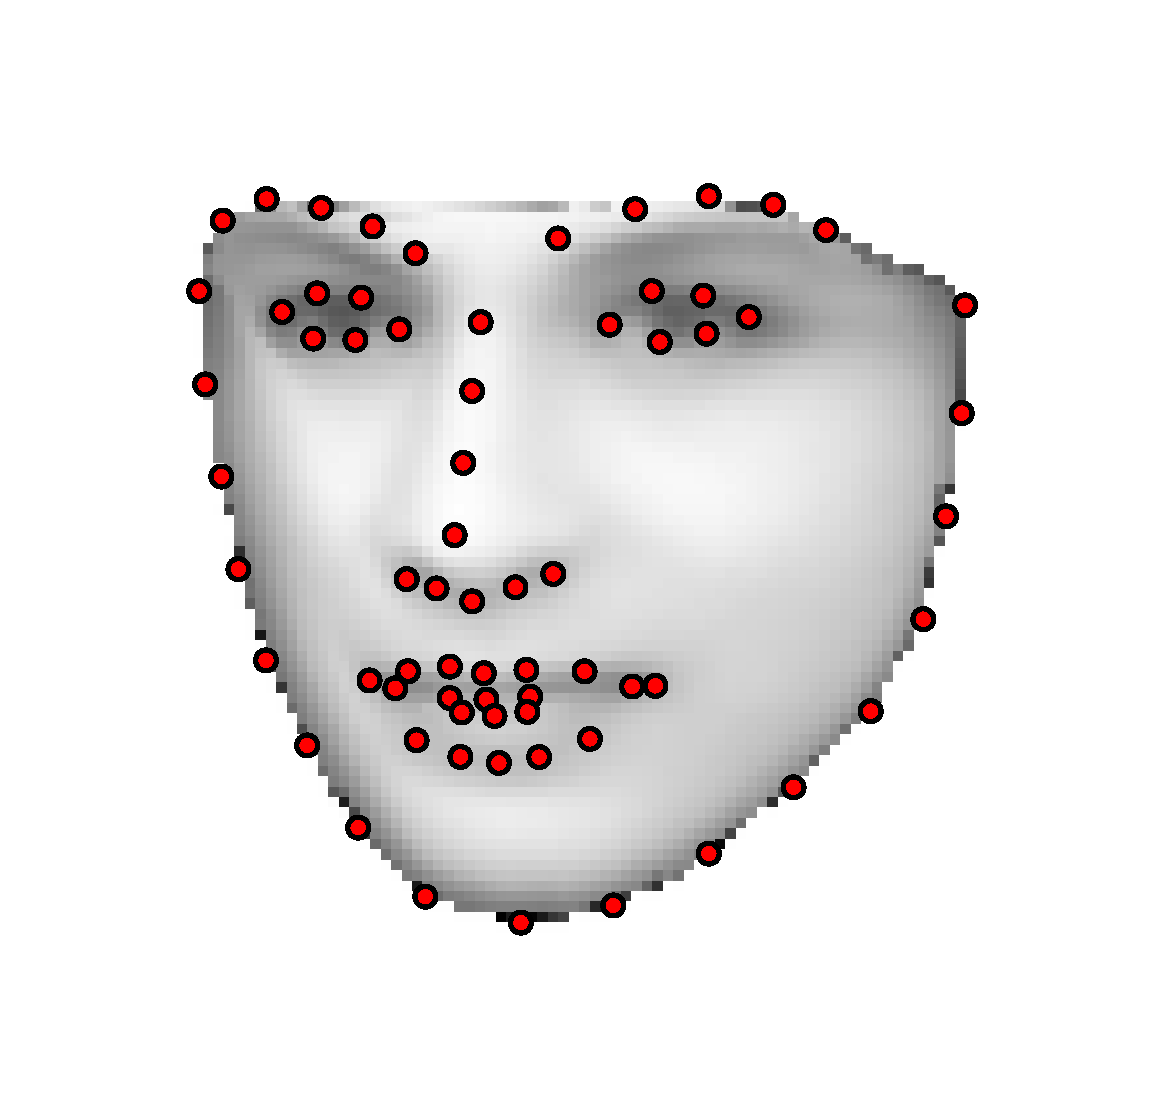
\includegraphics[width=\textwidth]{resources/Fig_dAAM/of_app}
%     \end{subfigure}
%     \caption{Dense Deformable Model}
%     \label{fig:models}
% \end{figure}

{\refstepcounter{steps}\label{sec:step4}\subsection*{Step 4: Dense and Patch-Based Deformable Models}}
% \subsection{Dense and Patch-Based Active Appearance Models}


\begin{figure}[b!]
    \centering
    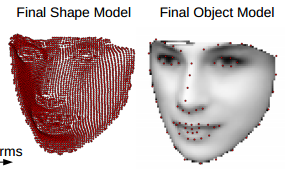
\includegraphics[width=0.45\textwidth]{resources/models}
    \caption{Exemplar dense shape models build for faces and ears. Dense shapes are presented as grid for better visualisation.}
    \label{fig:dense_models}
\end{figure}


The deformation fields obtained from Step~\ref{sec:step3} can be used to naturally build two different kinds of effective Active Appearance Models (AAMs) \cite{Cootes2001, Matthews2004}: \emph{dense} \cite{ramnath2008increasing, Amberg2009, anderson2014using} and \emph{patch-based} \cite{Tzimiropoulos2014}. The only difference between these two AAM formulations is on the way that the shape is represented and, thus, the manner in which the texture is sampled. Each one of them is suitable for object classes with specific properties. The dense AAM provides an exceptionally effective modeling and fitting for non-articulated objects, such as ears and faces, whose appearance has characteristic structures that spread all over their region (even if these structures cannot be consistently annotated). On the other hand, there exist other challenging object classes, such as arms and legs, that not only cannot be consistently annotated with landmarks, but their appearance is distinctive only on the object's outline and not in its interior region. Especially in the case of human body parts, they are almost always covered by clothes, which makes it impossible to construct robust texture models.

\paragraph{Dense Active Appearance Model} Since all the deformation fields acquired by Step~\ref{sec:step3} contain the same number of pixels, which are the same as in the reference frame, the spatial positions $\bm{x}_i=(x_i, y_i)$ of these pixels can be treated as point landmarks and the deformation fields as dense annotations of the object's shape. Consequently, building a dense shape model reduces to normalising these dense annotations with respect to a global similarity transform (typically using Procrustes Analysis) and applying PCA. A shape instance can be generated by the resulting shape model as:
\begin{equation}
    \bm{s}(\bm{p}) = \bm{\bar{s}} + \bm{S} \bm{p}
    \label{eq:shape_model}
\end{equation}
where $\bm{\bar{s}}$ is mean shape, and $\bm{S}$ and $\bm{p}$ are the shape bases and shape parameters, respectively.

By making explicit use of the one-to-one correspondence between pixels on the reference frame and on the deformation fields, the motion model of sparse holistic AAMs \cite{Cootes2001, Matthews2004} (piece-wise affine, thin-plates splines \cite{Bookstein1989}) is replaced by sampling all pixel values onto the reference frame. Let us define this sampling function, given a shape instance $\bm{s}(\bm{p})$, as $\mathcal{W}(\bm{s}(\bm{p}))$. Once the images have been warped, the texture model is obtained by applying PCA on them. A texture instance can be generated as:
\begin{equation}
    \bm{t}(\bm{c}) = \bm{\bar{t}} + \bm{T} \bm{c}
	\label{eq:tex_model}
\end{equation}
where $\bm{t}$ is the mean texture, and $\bm{T}$ and $\bm{c}$ are the texture bases and texture parameters, respectively.

Given a test image $\mathbf{I}$, the fitting process involves the minimisation of the following cost function:
\begin{equation}
    \arg\min_{\bm{p}, \bm{c}}\|\bm{I}(\mathcal{W}(\bm{s}(\bm{p}))) - \bm{t}(\bm{c})\|_2^2
	\label{eq:aam_cost}
\end{equation}
This optimisation problem is typically solved using the inverse-compositional Gauss-Newton algorithm, for which different variations have been proposed \cite{Matthews2004, Papandreou2008, Amberg2009, Tzimiropoulos2013, Alabort2014}. Note that the existence of the sampling function $\mathcal{W}()$ instead of a non-linear warping function has the advantage that all existing efficient gradient descent algorithms become exact.

\paragraph{Outline Patch-Based Active Appearance Model}
The object classes for which the interior appearance does not have specific structure are modeled using patch-based AAMs \cite{Tzimiropoulos2014} trained on a set of sparse landmarks. Especially for human body parts (arms, legs), we strongly believe that the points located to the outline of the object are more suitable compared to the internal ones that correspond to the skeleton joints, which are commonly used by current literature \cite{buehler2011upper,charles2013domain,pfister2015flowing,yang2013articulated}. 

The main differences between the patch-based and dense AAMs are that (a)~the densified shape instances are sub-sampled to include only the outline points, and (b)~the texture representation involves the sampling a neighbourhood around each point instead of a single pixel. Specifically, in order to build the outline sparse shape model, we simply select the outline points on the SVS reference frame. Then, by taking advantage of the dense correspondences obtained by Step \ref{sec:step3}, the shape model is trained in a similar way as in the dense case. Moreover, similar to the dense case, the texture model is built by sampling the image values from the sparse shape locations, i.e. $\mathcal{W}(\bm{s}(\bm{p}))$. However, contrary to dense AAMs, we sample a patch that is centred around each landmark point. These patches are then vectorised and concatenated in a single texture vector. Note that the optimisation process remains exactly the same.